\section{Dynamics of a Single Cell}
In this section the results of the numerical solutions for a single cell
using the three models presented above are discussed. All results were
obtained with a simple Forward-Euler scheme.

\subsection{Hodgkin \& Huxley}
The equations were integrated for \SI{10}{\milli\second} with a time step
$\Delta{t}=\SI{.01}{\milli\second}$ (\ie~1000 integrations steps) and an
initial potential $V_0=\SI{-7}{\milli\volt}$. The resulting action potential,
current densities and gating variables are plotted in \figref{fig:hh1}.

\begin{figure}[h]
    \centering
    \begin{subfigure}[h]{.3\textwidth}
        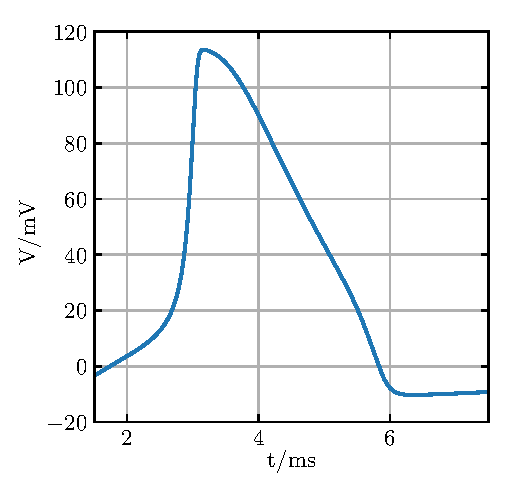
\includegraphics[width=\textwidth]{hh52-10ms-V}
        \label{fig:hh1V}
        \caption{Potential}
    \end{subfigure}
    \begin{subfigure}[h]{.3\textwidth}
        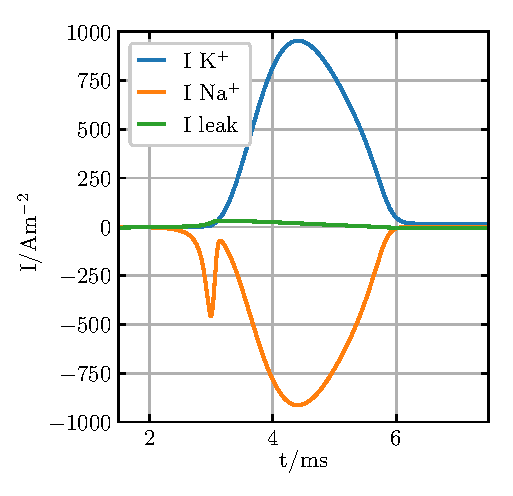
\includegraphics[width=\textwidth]{hh52-10ms-I}
        \label{fig:hh1I}
        \caption{Current Densities}
    \end{subfigure}
    \begin{subfigure}[h]{.3\textwidth}
        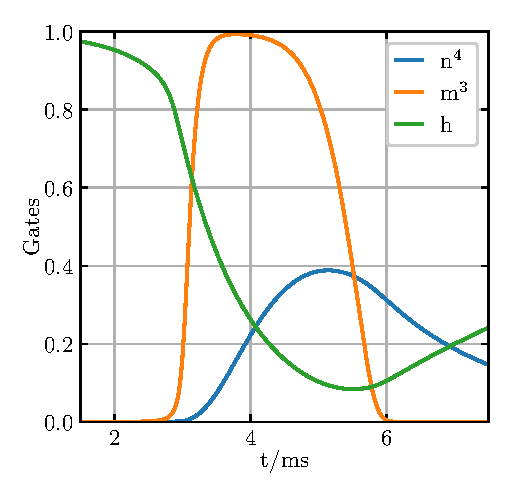
\includegraphics[width=\textwidth]{hh52-10ms-Gates}
        \label{fig:hh1Gates}
        \caption{Gating Variables}
    \end{subfigure}
    \label{fig:hh1}
    \caption{Results of integrating the H\&H model}
\end{figure}

The gating variables were initially all set to 0, yet at
$t=\SI{0}{\milli\second}$ the \ce{Na+} gate $h$ jumps directly to being almost
completely open ($h(t=0)=0.99$); however, the \ce{Na+} current is at this point
suppressed by the closed $m$ gate. The $h$ gate slowly closes up to
$t\approx\SI{5}{\milli\second}$ and then swings down more rapidly, while at the same
time the $m$ gate opens strongly and allows for influx of \ce{Na+} ions
(interesetingly yhe \ce{Na+} current exhibits a small seperate peak at
$t\approx\SI{5}{\milli\second}$ before rising up to its full strength). This
causes the membrane potential to rise up and become strongly positive. Shortly
after the quick opening of the $m$ gate, the \ce{K+} gate $n$ also opens,
allowing for an opposed \ce{K+} outflux causing the membrane potential to
eventually repolarize.

The resulting action potential resembles qualitatively the results depicted in
fig.~12 in [HH52] \todo{add paper to literature and cite properly}. An even
better fit is achieved when integrating the system for \SI{40}{\milli\second}
with and initial value of $V_0=\SI{-30}{\milli\volt}$, as depicted in fig.~22
in [HH52] (see \figref{fig:hh2}).

\begin{figure}[h]
    \centering
    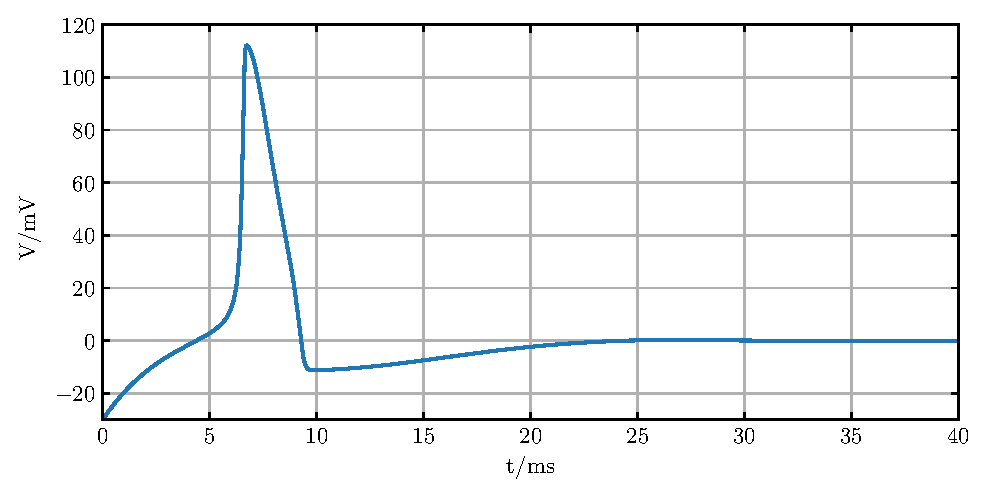
\includegraphics[width=.75\textwidth]{hh52-40ms}
    \label{fig:hh2}
    \caption{H\&H for \SI{40}{\milli\second}; note the hyperpolarization}
\end{figure}

Another interesting effect can be observed when adding an additional source
current to equation \eqref{eq:cap}, \ie:
\begin{equation*}
    C\,\dv{V}{t}=-\sum_{s}I_{s} + I_{\mathrm{source}}
\end{equation*}
which causes the membrane potential to depolarize again after repolarization
with a constant rate as depicted in \figref{fig:hh3}. Note, that \todo{minimal
firing rate for given source current}

% \begin{figure}[h]
%     \centering
%     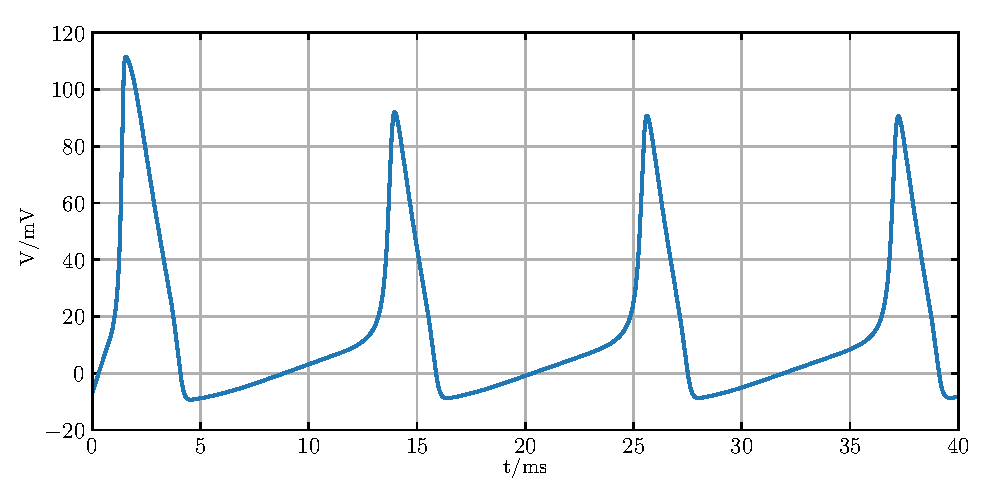
\includegraphics[width=.5\textwidth]{hh52-40ms-10nA}
%     \label{fig:hh3}
%     \caption{}
% \end{figure}


% vim: set ff=unix tw=79 sw=4 ts=4 et ic ai :
